\documentclass[11pt,a4paper]{article}
\usepackage[utf8x]{inputenc}
\usepackage{graphicx}
\usepackage{esdiff}
\usepackage[english]{babel}
\usepackage{color}
\usepackage{float}
\usepackage{enumitem}
\usepackage{epstopdf}
\usepackage{afterpage}
\usepackage{caption}
\usepackage{subcaption}
\captionsetup[table]{oneside , margin = {2cm, 0cm},
	justification=RaggedRight, singlelinecheck = false }
\usepackage{subcaption}
\usepackage{mathtools}
\usepackage{multicol}
\usepackage{algorithm2e}
\usepackage{microtype}
\usepackage{titling}
\usepackage{amsmath}
\usepackage{verbatim}
\usepackage[colorlinks=true]{hyperref} % the option is there to remove the square around links which is what I don't like.
\usepackage{comment}
\usepackage{perpage} 
\MakePerPage{footnote} % Reset the footnote counter perpage. may require to run latex twice.
\usepackage{commath} % for absolute value
\usepackage[margin=2cm]{geometry} % This is here to fit more text into the page.

\setcounter{secnumdepth}{1}  % This removes the numbering from the subsections.
% If you want the numbering of the subsection level just remove this line
\usepackage{titling}
\newcommand{\subtitle}[1]{%
	\posttitle{%
		\par\end{center}
	\begin{center}\large#1\end{center}
	\vskip0.5em}%
}

\setlength{\parindent}{0pt} % No indentation for paragraphs. Because that is just old.
\setlength{\parskip}{\baselineskip} % Instead use vertical paragraph spacing.

\fontencoding{T1} % the better font encoding.

\begin{document}	
\section*{Homework 1  \hfill Giorgio Checola}
\subsection{Exercise 1}
\begin{figure}[H]
\centering 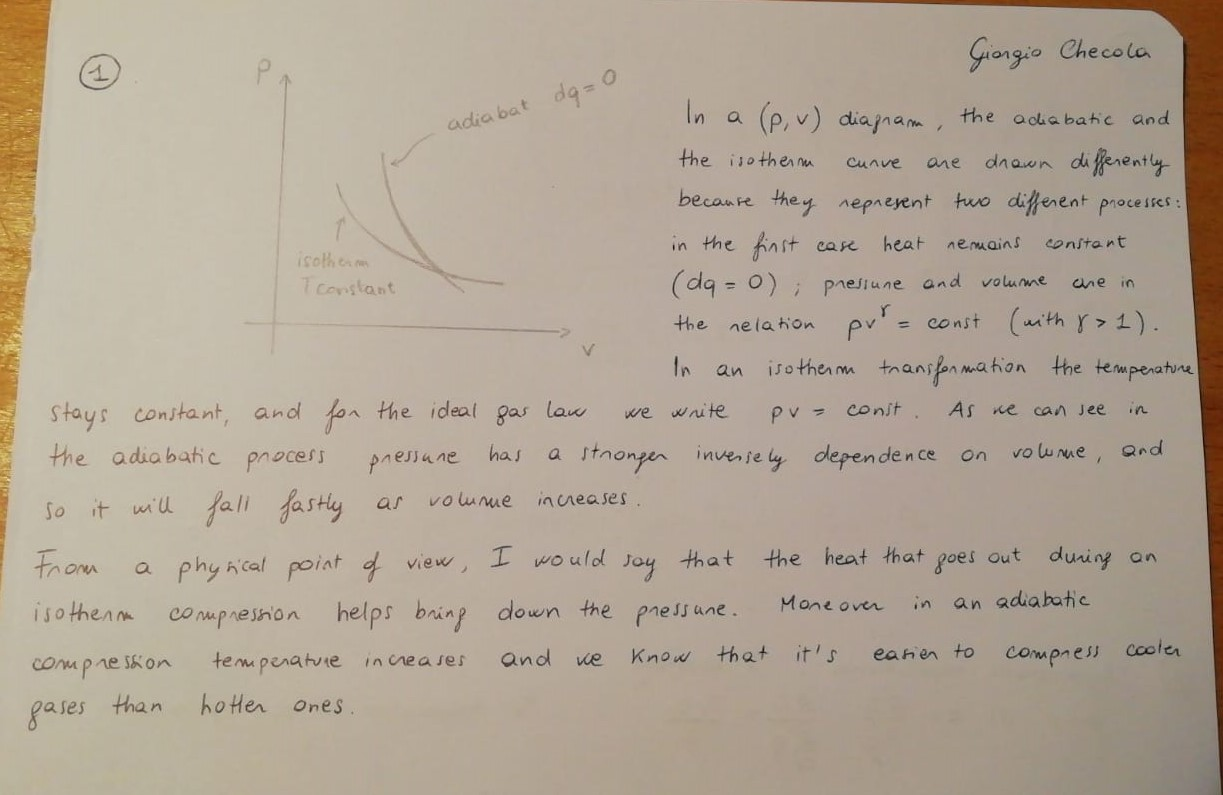
\includegraphics[width=150mm]{images/es1.JPEG}
\end{figure}
\subsection{Exercise 2}
\begin{figure}[H]
	\centering 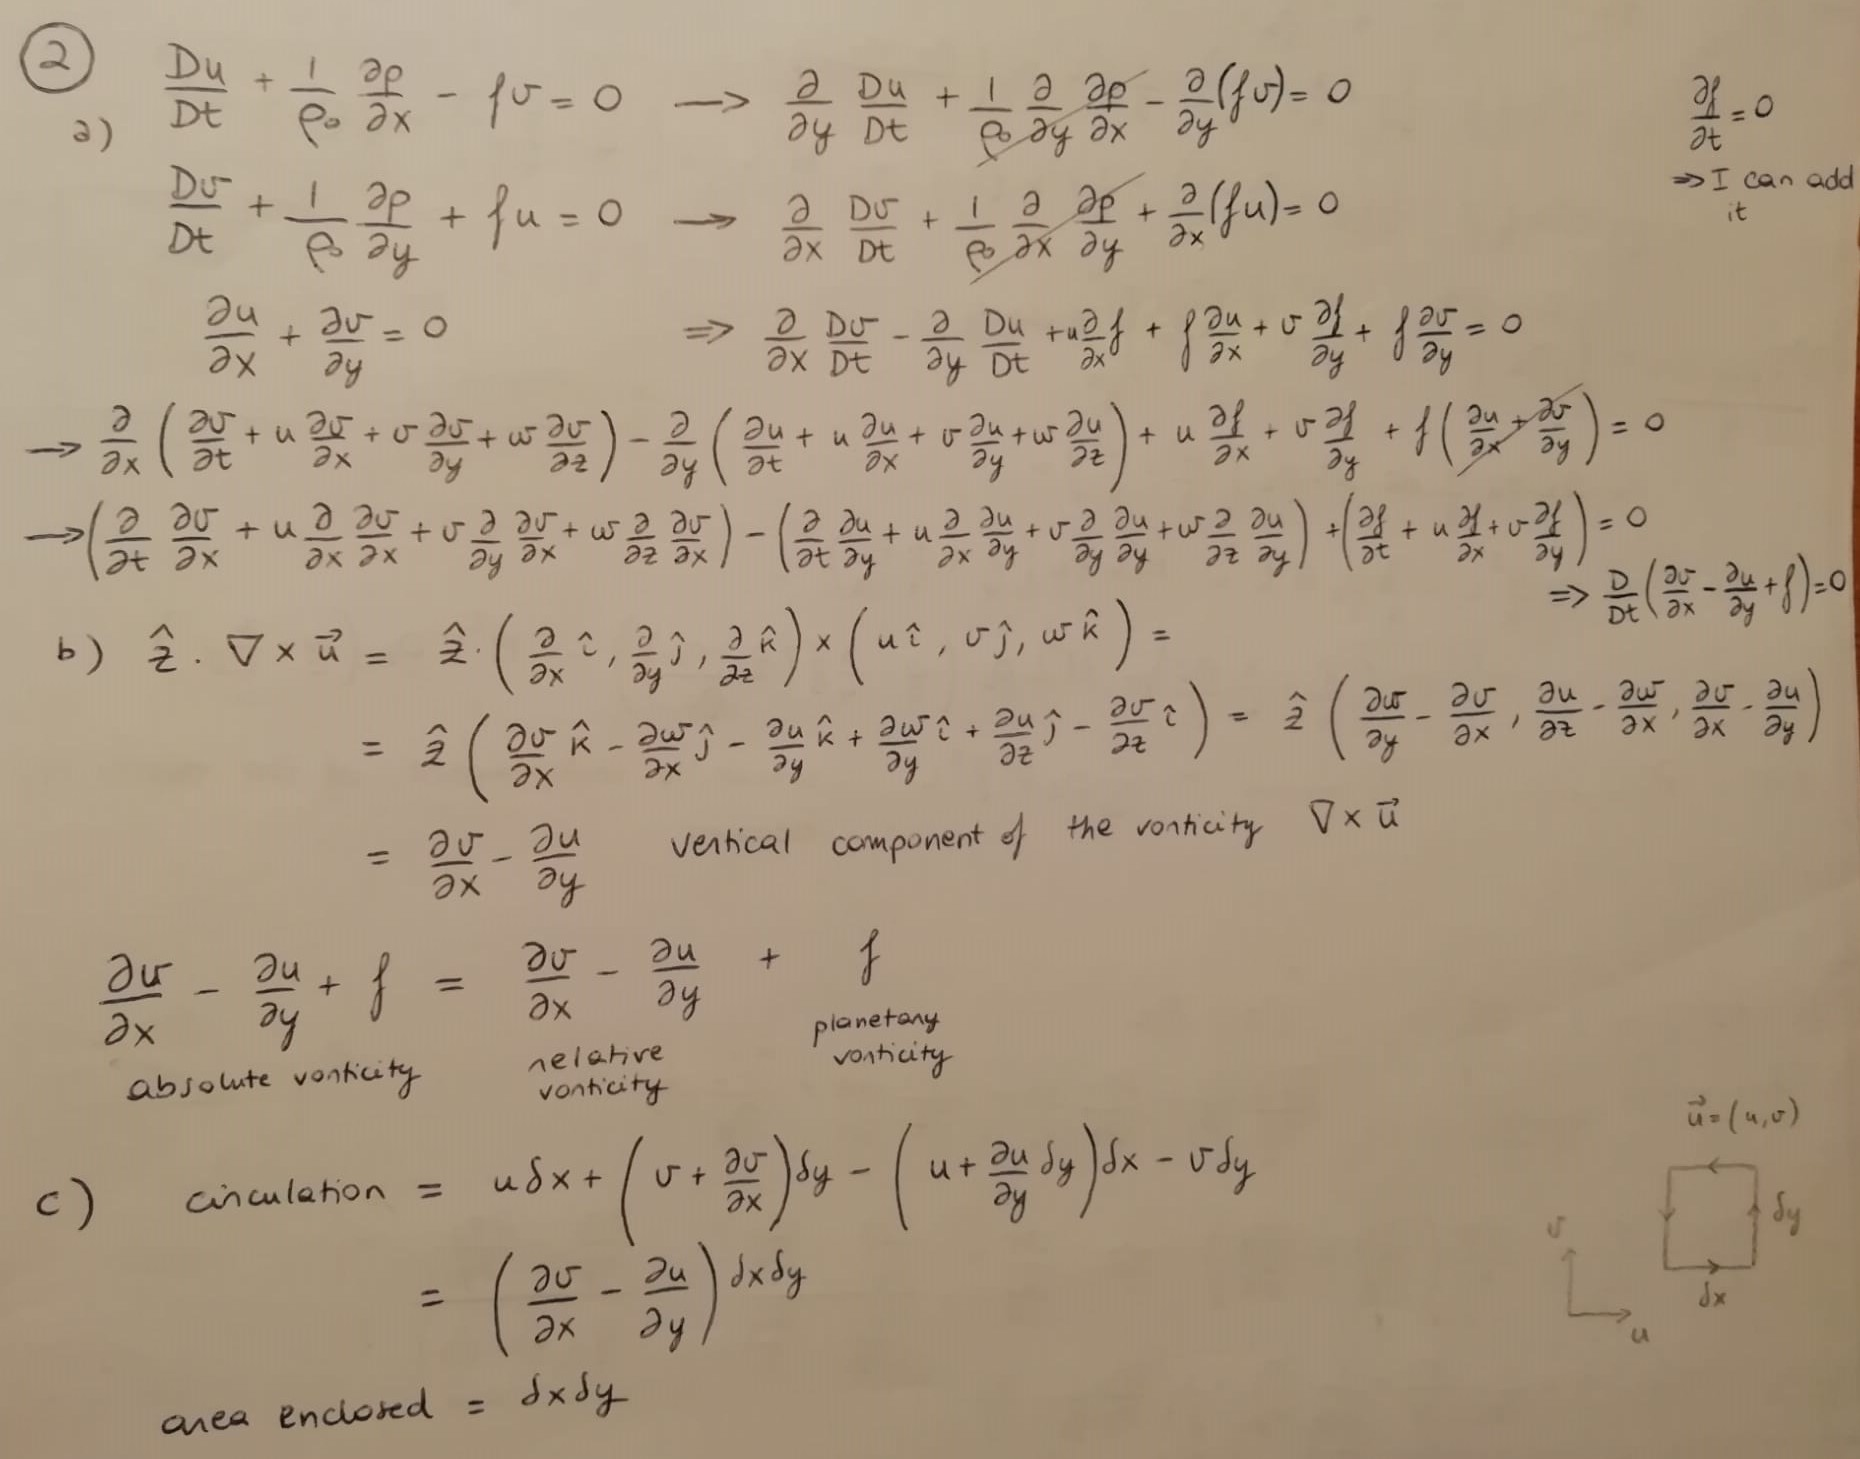
\includegraphics[width=150mm]{images/es2.JPEG}
\end{figure}
\subsection{Exercise 3}
\begin{figure}[H]
	\centering 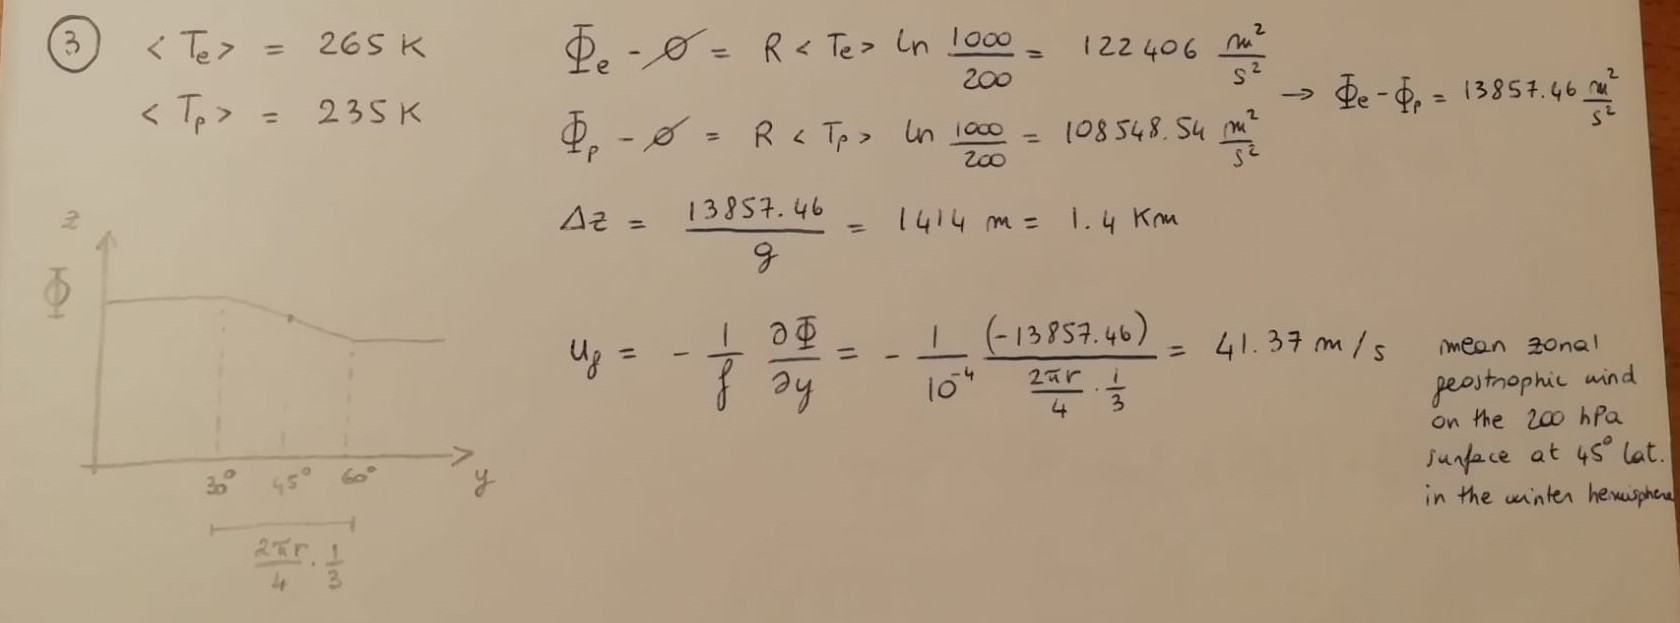
\includegraphics[width=150mm]{images/es3.JPEG}
\end{figure}
\subsection{Exercise 4}
\begin{figure}[H]
	\centering 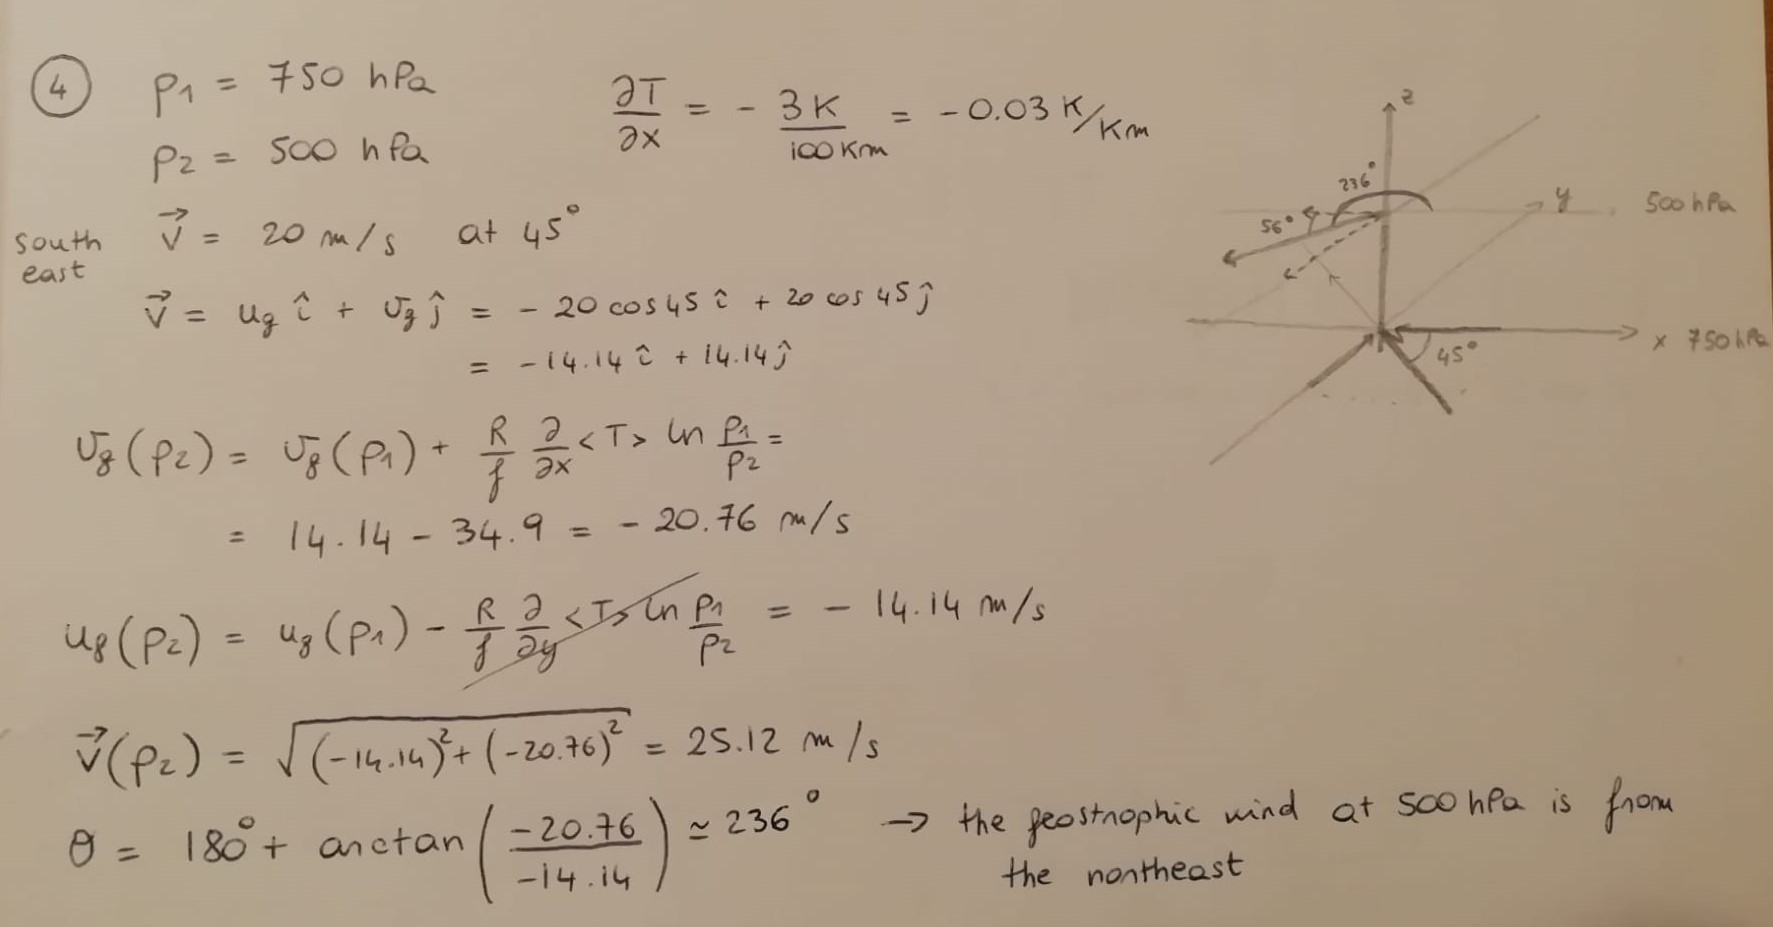
\includegraphics[width=150mm]{images/es4.JPEG}
\end{figure}
\subsection{Exercise 5}
\begin{figure}[H]
	\centering 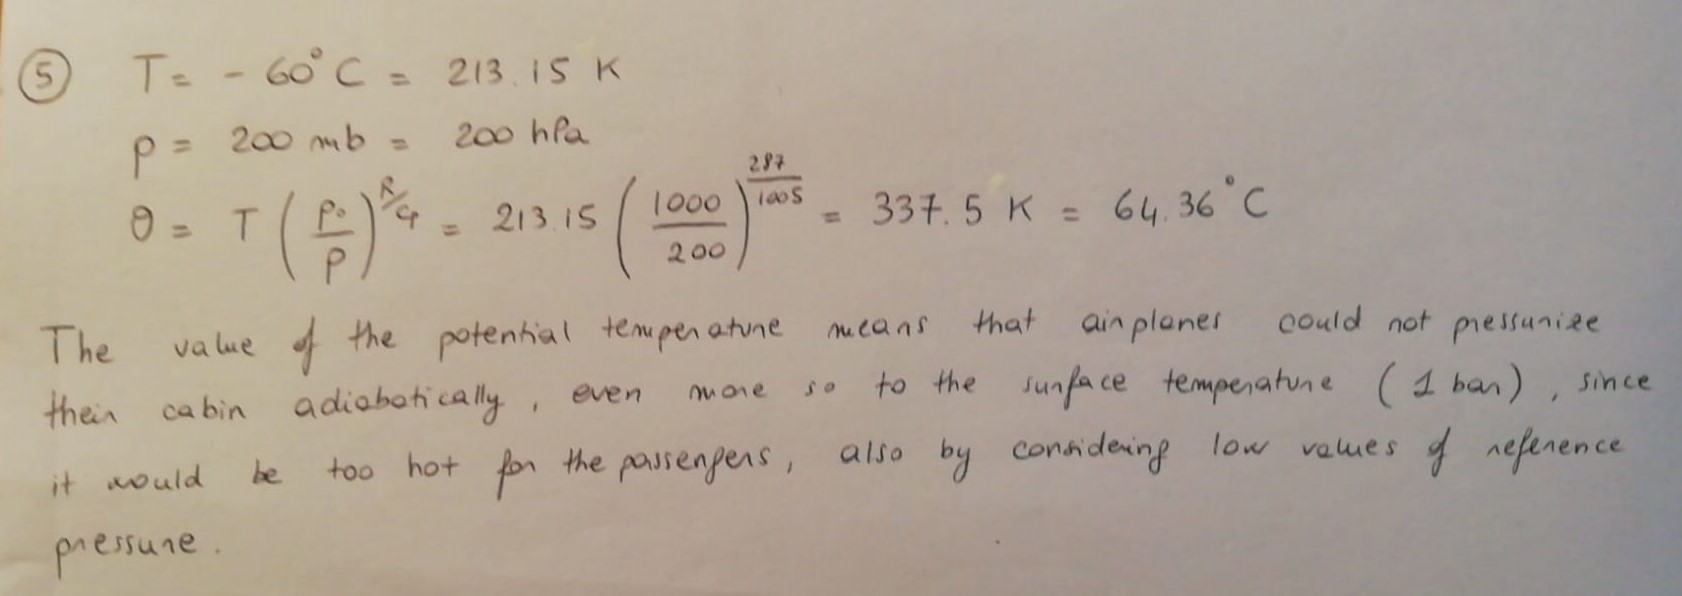
\includegraphics[width=150mm]{images/es5.JPEG} 
\end{figure}
\subsection{Exercise 6}
\begin{figure}[H]
	\centering 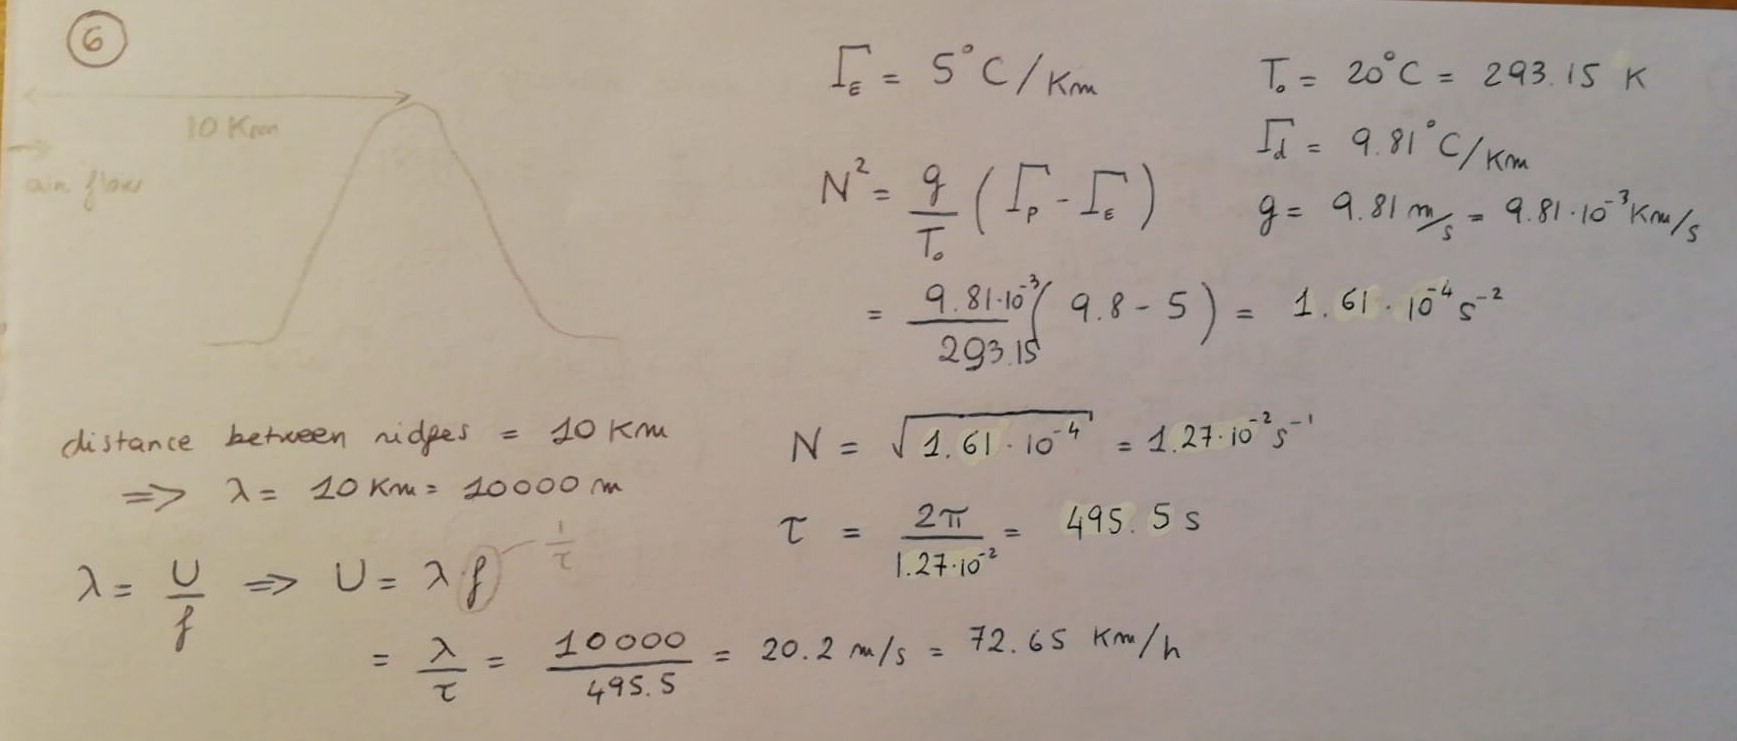
\includegraphics[width=150mm]{images/es6.JPEG}
\end{figure}
\subsection{Exercise 7}
\begin{figure}[H]
	\centering 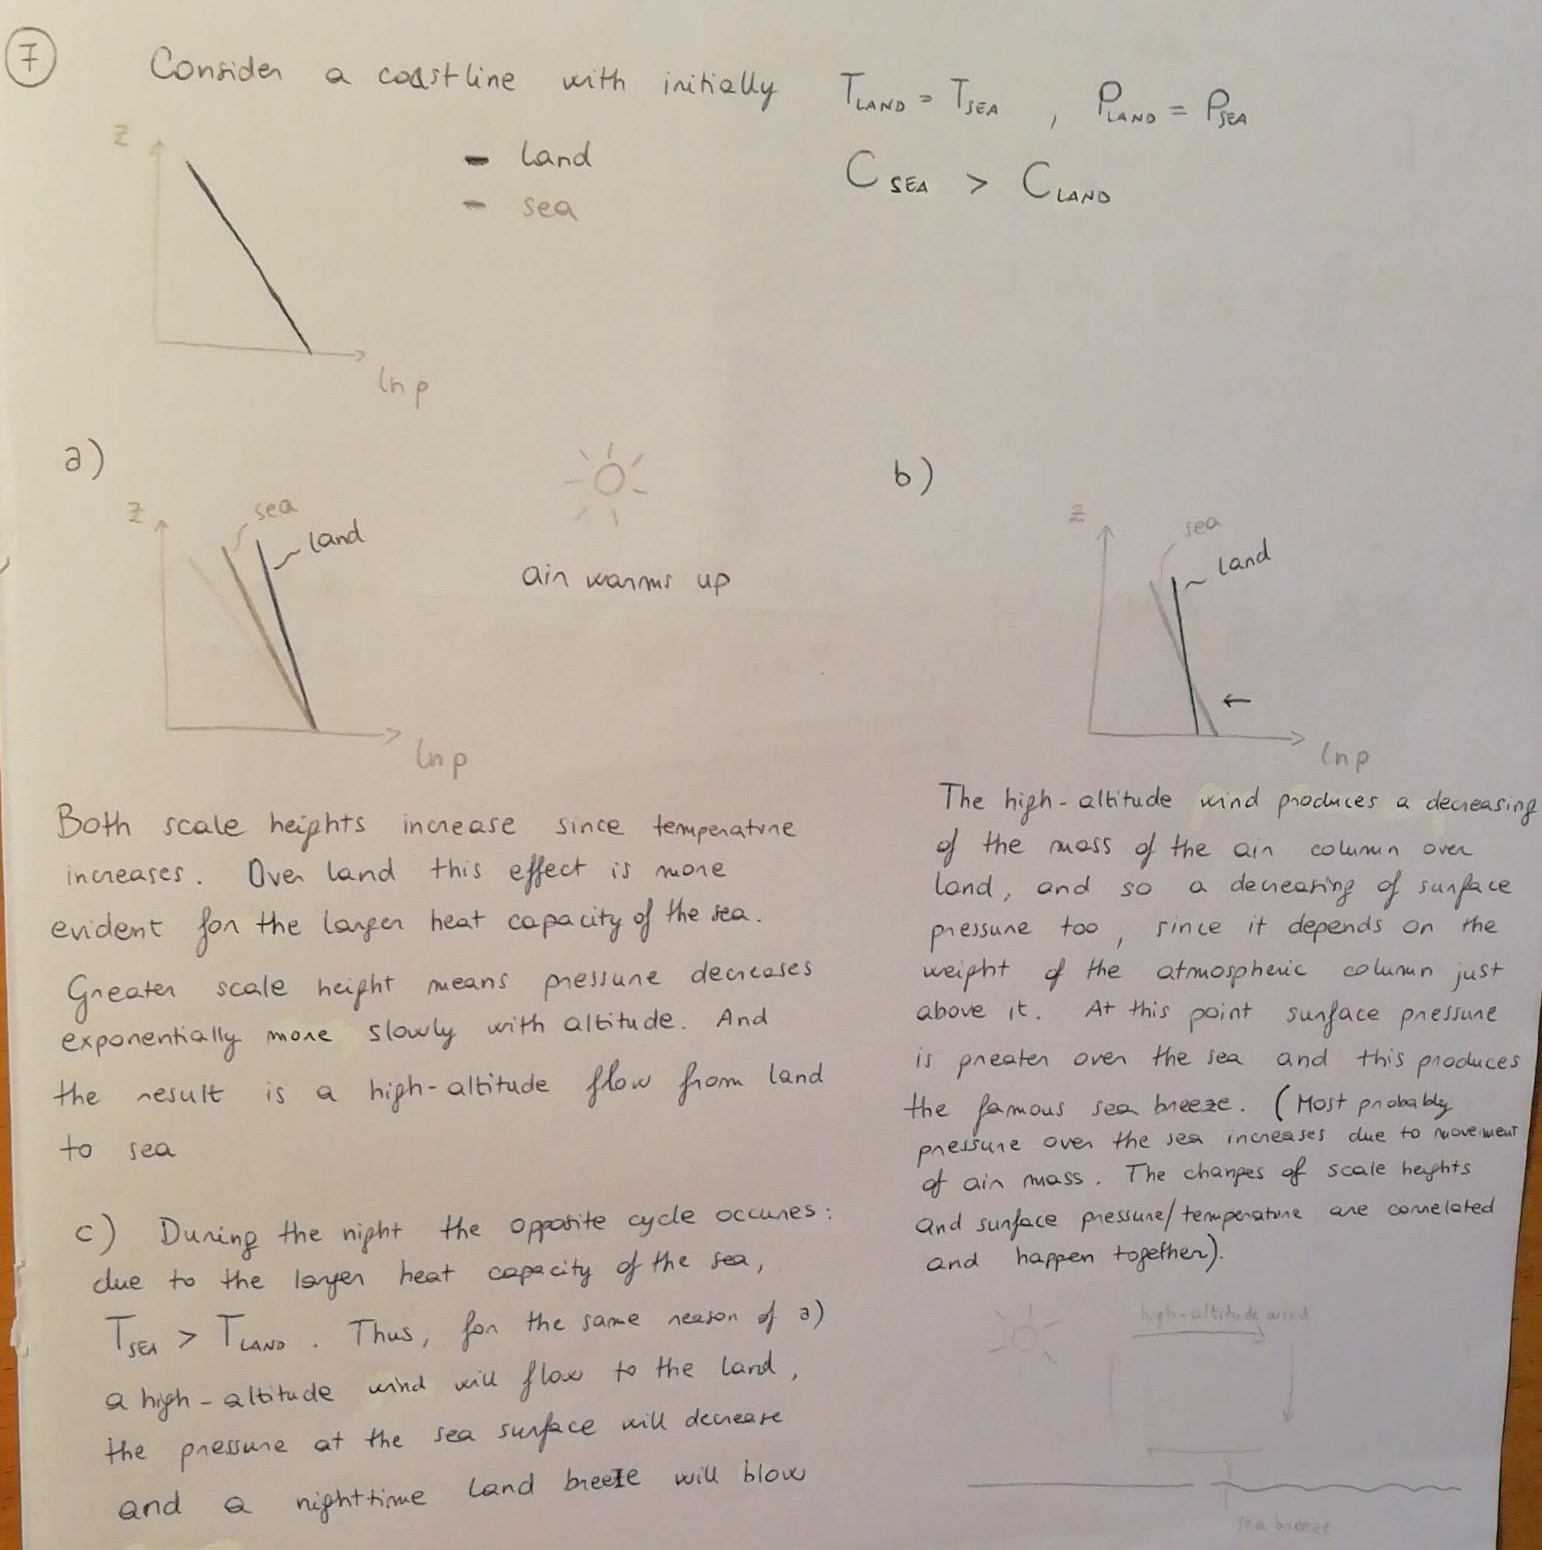
\includegraphics[width=150mm]{images/es7.JPEG}
\end{figure}
\subsection{Exercise 8}
\begin{figure}[H]
	\centering 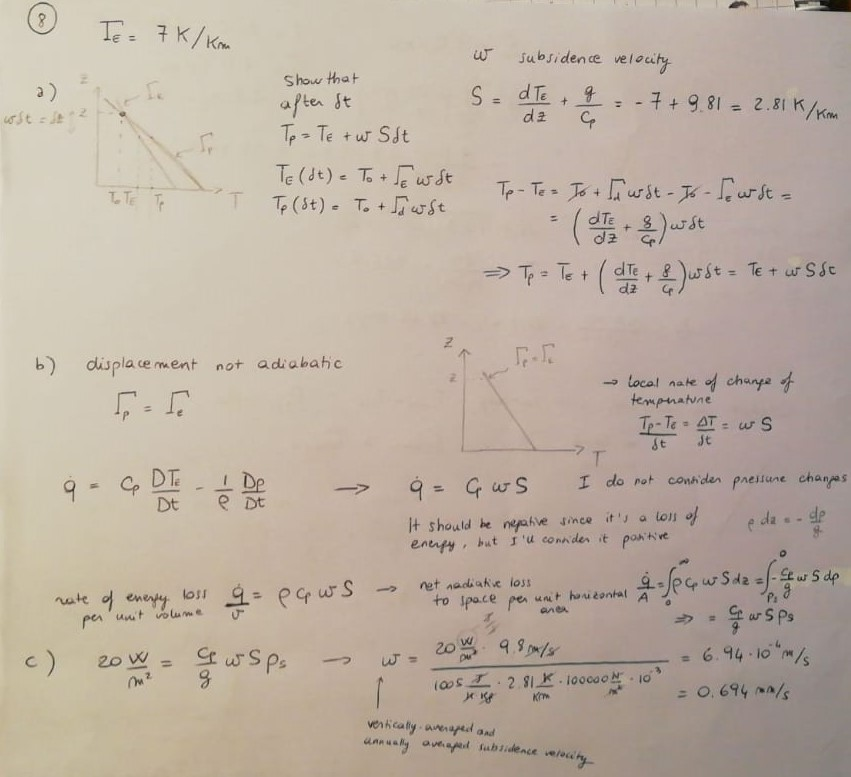
\includegraphics[width=150mm]{images/es8.JPEG}
\end{figure}

\end{document}